\documentclass[table, 12pt]{article}
\usepackage{graphicx}
\usepackage[T1]{fontenc}
\usepackage{tocloft}
\usepackage{caption}
\usepackage{hyperref}
\usepackage{booktabs}
\usepackage{listings}
\usepackage{pdfpages}
\usepackage{pdflscape}
\usepackage{textpos}
\usepackage{scrhack}
\usepackage{xcolor}
\usepackage{float}
\usepackage{longtable}
\usepackage{enumitem}
\usepackage{tasks}
\usepackage{tabularx}
\usepackage{titlesec}
\usepackage{listing}
\usepackage{graphicx}


\titleformat{\paragraph}
{\normalfont\normalsize\bfseries}{\theparagraph}{1em}{}
\titlespacing*{\paragraph}
{0pt}{3.25ex plus 1ex minus .2ex}{1.5ex plus .2ex}

\begin{document}
\begin{titlepage}
    \centering
    {\scshape\large AY 2020/2021 \par}
    \vfill
    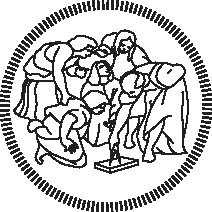
\includegraphics[width=100pt]{assets/logo-polimi-new}\par\vspace{1cm}
    {\scshape\LARGE Politecnico di Milano \par}
    \vspace{1.5cm}
    {\huge\bfseries Middleware Technologies\\Contact Tracing with IoT Devices\par}
    \vspace{2cm}
    {\Large {Federico Armellini\quad Luca Pirovano\quad Nicolò Sonnino}\par}
    \vfill
    {\large Professor\par
        Luca \textsc{Mottola}}
    \vfill
    {\large \textbf{Version 1.0}\\ \today \par}
\end{titlepage}
\hypersetup{%
    pdfborder = {0 0 0}
}
\thispagestyle{plain}
\pagenumbering{gobble}
\mbox{}
\newpage
\pagenumbering{roman}
\tableofcontents
\newpage
\pagenumbering{arabic}
\section{Introduction}
\subsection{Description of the project}
People roaming in a given location carry IoT devices.

The devices use the radio as a proximity sensor. Every time
two such devices are within the same broadcast domain, that is, at 1-hop distance from each other, the two
people wearing the devices are considered to be in contact.

The contacts between people’s devices are
periodically reported to the backend on the regular Internet. Whenever one device signals an event of interest,
every other device that was in contact with the former must be informed.


\section{Solution Overview}

\subsection{General Architecture}

\begin{figure}[!ht]
    \centering
    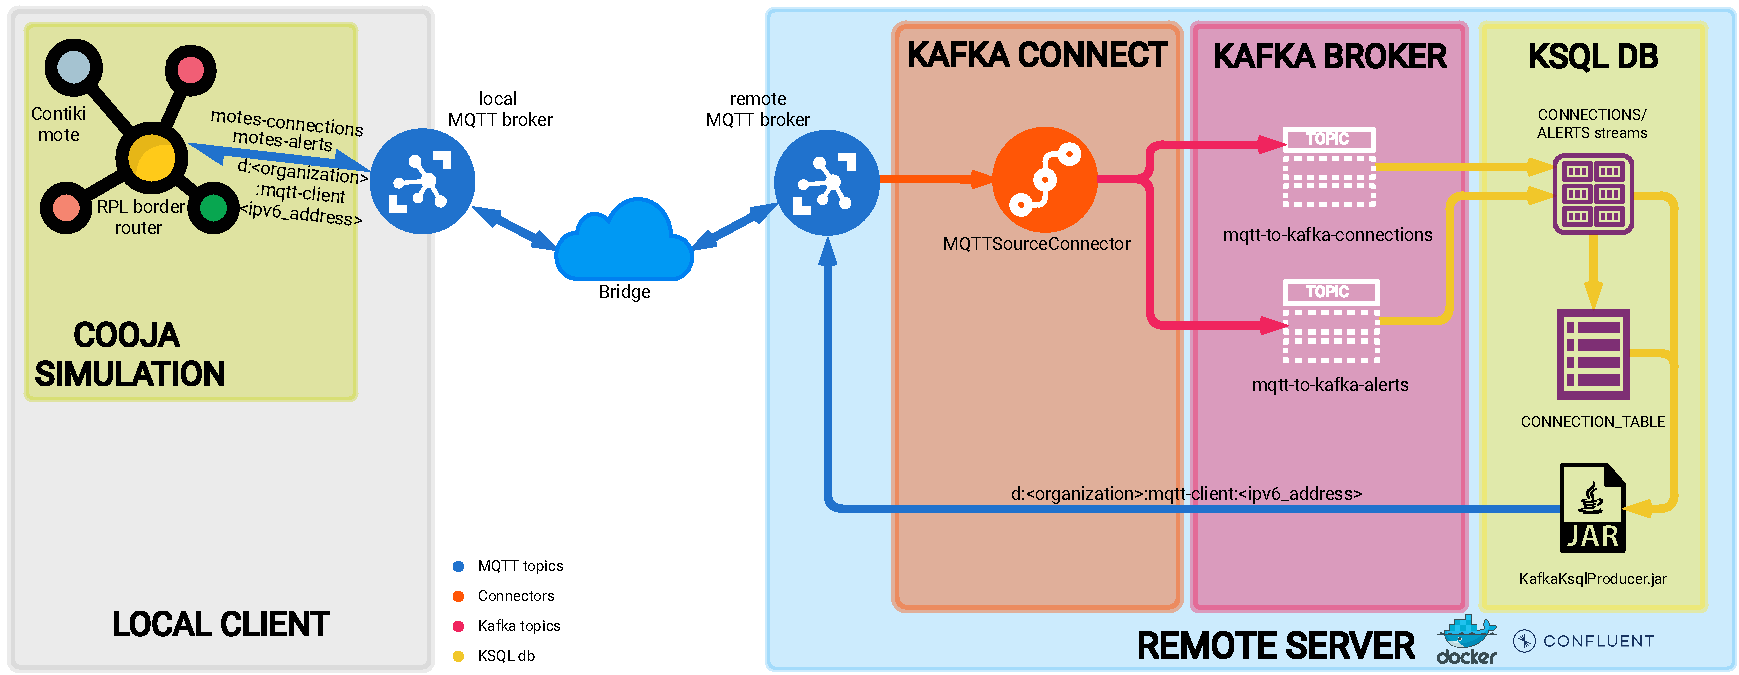
\includegraphics[width=\textwidth]{assets/middleware.pdf}
\end{figure}

The project consists into an integration of Contiki-NG motes with Apache Kafka using Confluent Platform and Docker.

Confluent was used for an easy management of Apache Kafka while Docker was utilized for deploying Confluent Platorm and Apache Kafka into containers (increasing scalability and manageability of the infrastructure).
\newpage
\paragraph{Platforms}
\begin{itemize}
    \item \href{https://kafka.apache.org/}{\textbf{Apache Kafka}}
    \item \href{https://docs.confluent.io/platform/current/overview.html}{\textbf{Confluent Platform}}
    \item \href{https://www.contiki-ng.org/}{\textbf{Contiki-NG}}
    \item \href{https://www.docker.com/}{\textbf{Docker}}
    \item \href{https://www.confluent.io/product/ksql/}{\textbf{KSQL}}
\end{itemize}

\paragraph{Protocols}
\begin{itemize}
    \item \href{https://mqtt.org/}{\textbf{MQTT}}
    \item \href{https://tools.ietf.org/html/rfc6550}{\textbf{RPL}}
    \item \href{https://www.rfc-editor.org/ien/ien71.pdf}{\textbf{UDP}}
\end{itemize}

\paragraph{Components}
The following list explains each component of the workflow:
\begin{itemize}
    \item \textbf{Contiki-NG motes}: motes running \texttt{contact-tracing.c} program and emulated in the COOJA simulator or compiled natively.

          They use RPL (Routing Protocol for Low-Power and Lossy Networks) protocol in order to exchange messages between them and MQTT (Message Queue Telemetry Transport) protocol for communicating with the middleware.
          Each mote runs three processes:
          \begin{enumerate}
              \item \underline{Broadcast}: this process fires a broadcast UDP message containing the mote's client ID at regular intervals.
              \item \underline{Broadcast receiver}: process responsible for receiving clients IDs via UDP from other motes and inserting them into the MQTT queue buffer in order to publish them later.
              \item \underline{MQTT main process}: main process, it manages the whole MQTT workflow: it publishes to \texttt{mqtt-to-kafka-connections} and \\ \texttt{mqtt-to-kafka-alerts} MQTT topics both the motes' connection between each other and events called alerts at random intervals. It also subscribes to the \texttt{kafka-to-mqtt-alerts} topic listening to incoming events.
          \end{enumerate}
    \item \textbf{RPL border router}: mote acting as a router for sharing messages between motes and outside connections.
    \item \textbf{MQTT broker}: it is the component handling messages from clients and topics, it is deployed both on the local client and on the remote server. They are both connected: the local one uses bridge mode and forwards every MQTT event to the remote one (very useful when using IPv6 or if the local client is running into a Virtual Machine).
    \item \textbf{MQTTSourceConnector}: Confluent connector (using Kafka Connect functionality) which reads from a MQTT topic (connection and alert in this case) and writes each publish on a Kafka one.
    \item \textbf{Kafka broker}: broker managing Kafka topics and connectors and interfacing with the KSQL system.
    \item \textbf{KSQLdb}: KSQL is a technology developed by Confluent, it allows to keep Kafka streaming versatility and it combines with a SQL language. \\It implements two different structures:
          \begin{enumerate}
              \item \underline{Streams}: continuous queries of streams of data in Kafka topics, they insert the content into the KSQLdb in order to store data. In the implementation two streams were instantiated: one for connections and one for alerts.
              \item \underline{Tables}: tables are views of streams and represents a collection of evolving facts. Every column specified into the table has a related value from the stream/table used for its creation. The main advantage of using KSQL tables is that updated values coming from streams are overwritten over the previous ones effectively avoiding duplications or outdated values. A table is used for storing connections between a node and the other ones.
          \end{enumerate}
    \item \textbf{KafkaKsqlProducer.jar}: Java program which creates two streams (CONNECTIONS and ALERTS), defines a table (CONNECTION\_TABLE) and instantiates a Kafka producer. Whenever an alert is received into the stream, the jar queries the CONNECTION\_TABLE (continuously updated by the CONNECTION stream) with the client ID contained into the message. The results are client IDs connected previously with that mote and they are used for each ProducerRecord wrote by the Kafka producer and sent to the "kafka-to-mqtt-alerts".
    \item \textbf{MQTTSinkConnector}: Equivalent of the MQTTSourceConnector, it receives messages from a Kafka topic and writes on a MQTT one.

\end{itemize}


\subsection{Flow of execution}

\subsection{Assumptions}
\begin{enumerate}[label=\textbf{A\arabic*:}]
    \item The IoT devices may be assumed to be constantly reachable, possibly across multiple hops, from a single static IoT device that acts as a IPv6 border router, that is, you don’t need to consider cases of network partitions.
    \item The IoT part may be developed and tested entirely using the COOJA simulator. To simulate mobility, you may simply move around nodes manually.
    \item Notification at a target device may be accomplished in simple ways, for example, by turning on a LED or printing something out on the serial console.
    \item Two IoT devices had a contact if they were reachable at 1-hop distance during a whole minute.
\end{enumerate}


\end{document}